\begin{frame}
    \frametitle{Fuzzing and RL}
    \begin{figure}
        \centering
        \begin{tikzpicture}[
                auto,
                box/.style = {
                        draw,rounded corners,blur shadow,fill=white,
                        align=center,text width=3cm,
                    },
            ]
            \node [box] [] (fuzzer) {Fuzzer(AFL, AFL++, ...)};
            \node [box] [below left = 3mm and 1.5cm of fuzzer] (state) {Branch count, crash, ...};
            \node [box] [below right = 3mm and 1.5cm of state] (program) {Program};
            \node [box] [below right = 3mm and 1.5cm of fuzzer] (seed) {Seed queue, mutation, ...};

            \path (fuzzer.south east) edge[cfgedge, bend left] (seed.north west);
            \path (seed.south west) edge[cfgedge, bend left] (program.north east);
            \path (program.north west) edge[cfgedge, bend left] (state.south east);
            \path (state.north east) edge[cfgedge, bend left] (fuzzer.south west);
        \end{tikzpicture}
    \end{figure}
    \begin{figure}
        \centering
        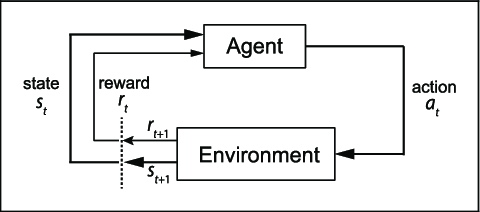
\includegraphics[height=0.3\textheight]{figs/rl.png}
    \end{figure}
\end{frame}